\subsection{Simulation RANS}

La méthode RANS (Reynolds-Averaged Navier-Stokes equations) consiste à appliquer un opérateur de moyenne statistique aux équations de Navier-Stokes. Le système d'équations ainsi obtenu est fermé par un modèle de turbulence [100]. Cette méthode permet de décrire la dynamique des grandeurs moyennes de l'écoulement. Initialement réservée aux écoulements stationnaires, une extension de la méthode RANS, appelée URANS (Unsteady-Reynolds-Averaged Navier-Stokes equations), existe pour les écoulements instationnaires. L'approche RANS est très intéressante pour obtenir le champ moyen dans les écoulements en des temps de restitution très courts. De ce fait, elle est très utilisée dans l'industrie pour simuler des écoulements turbulents. Toutefois, la méthode RANS n'est pas capable de représenter les interactions entre les structures qui sont à l'origine du bruit de jet. Il est donc nécessaire d'utiliser un modèle supplémentaire. Par exemple, les méthodes regroupées sous l'appellation SNGR (Stochastic Noise Generation and Radiation en anglais) [8] peuvent être utilisées. Elles consistent à déterminer un champ de vitesse turbulent à partir du spectre d'énergie turbulente de la simulation RANS. Ce champ de vitesse est ensuite employé pour construire les sources acoustiques.

\begin{figure}[h!]
 \centering
 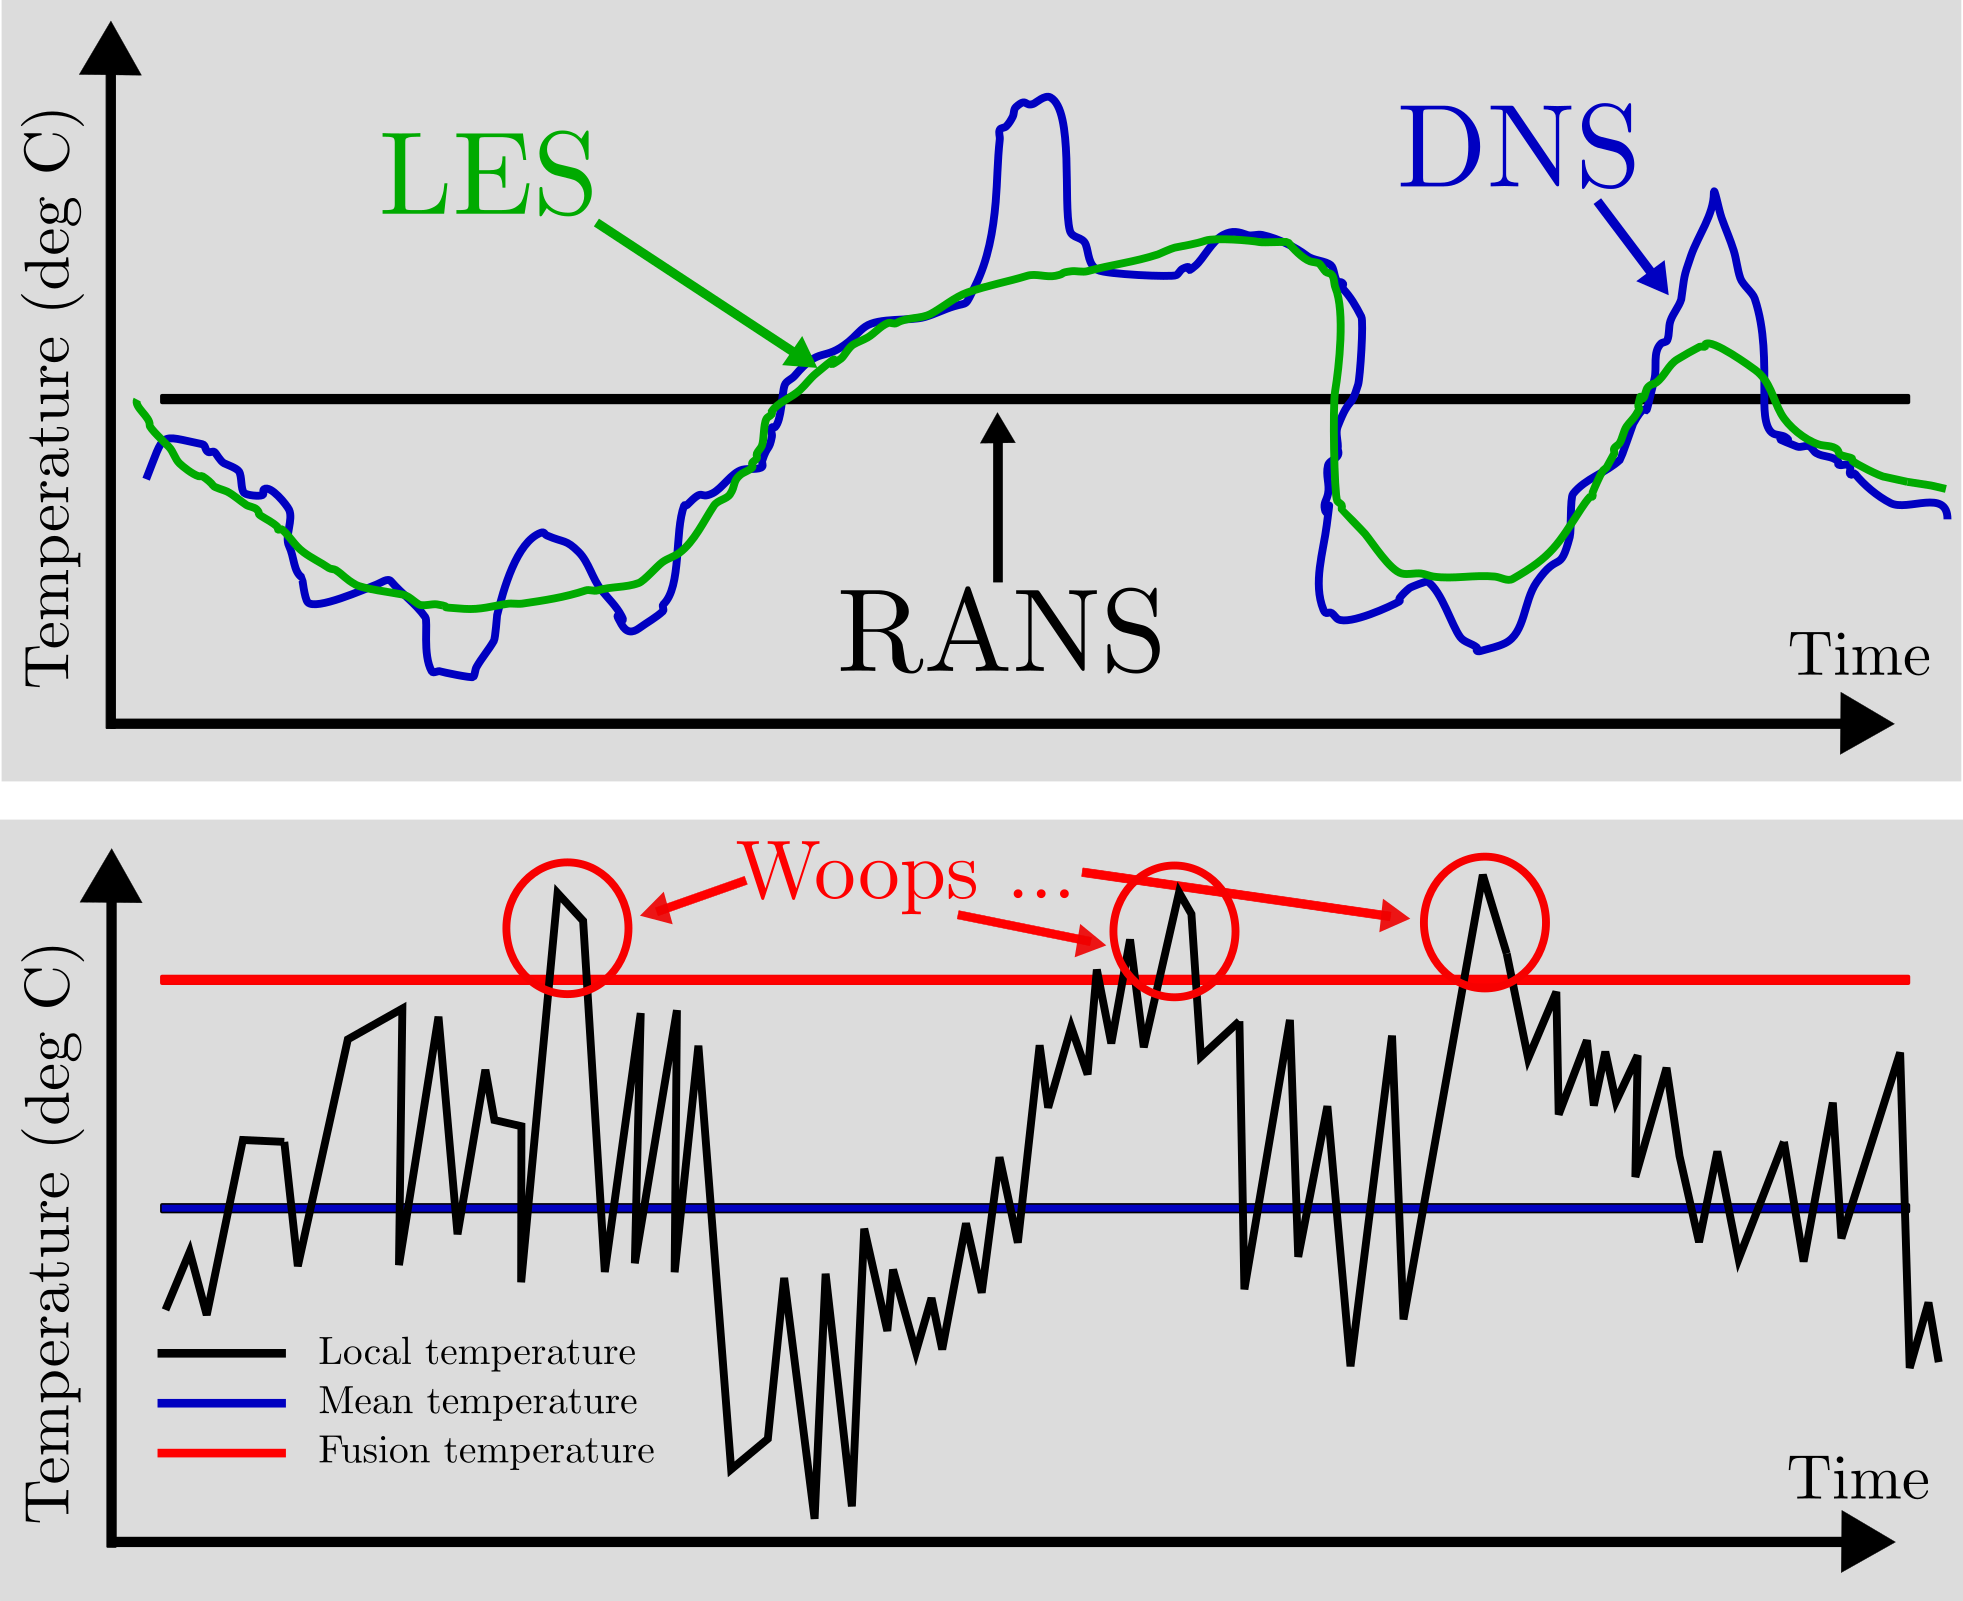
\includegraphics[width=1.0\linewidth]{chapter1_introduction/pictures/les_rans_dns.png}
 \vspace{-2ex}
 \caption{IXV spatial navette by esa}
  \vspace{2ex}
 \label{rans}
\end{figure}
